%\documentclass[twocolumn]{scrartcl}
\documentclass[parskip=true]{scrartcl}
\usepackage[utf8]{inputenc}
\usepackage{booktabs}
\usepackage{graphicx}
\graphicspath{ {img/} }
\usepackage{bm}
\usepackage{amsmath}
%\usepackage{parskip}
\usepackage{verbatim}
\usepackage{url}
\usepackage{enumitem}
\usepackage{float}
%\usepackage{subfig}
\usepackage{algorithm}
\usepackage{algorithmic}
\usepackage{subcaption}

\title{k-means clustering of multivariate data}
\subtitle{Parallel Computations for Large Scale Problems\\ SF2568}
\author{Kristófer Hannesson hannesso@kth.se\\Jökull Jóhannsson jokull@kth.se}
\date{\today}

\begin{document}

\maketitle

\section{Problem description}
% k-means clustering is an approach to cluster analysis which aims to partition a given data set into k clusters where each data point belongs to the nearest cluster prototype. Here a cluster prototype is the mean vector of the data points belonging to that cluster. Intuitively this method partitions the input space into Voronioi cells .

Given a set of data points $(\bm{x}_1, \bm{x}_2, ..., \bm{x}_n)$ in a d-dimensional input space, k-means clustering aims to partition the $n$ observations into $k$ sets $\bm{S} = \{S_1, S_2, ..., S_k\}$ such that the within-cluster sum of squares is minimized. The objective is therefore to find:

\begin{equation}
    \underset{\mathbf{S}} {\operatorname{arg\,min}}  \sum_{i=1}^{k} \sum_{\mathbf x \in S_i} \left\| \mathbf x - \boldsymbol\mu_i \right\|^2 
\end{equation}

where $\boldsymbol\mu_i$ is the mean of points in $S_i$. Intuitively this method partitions the input space into Voronioi cells as shown in figure \ref{fig:voronoi}.

\begin{figure}[h]
    \centering
    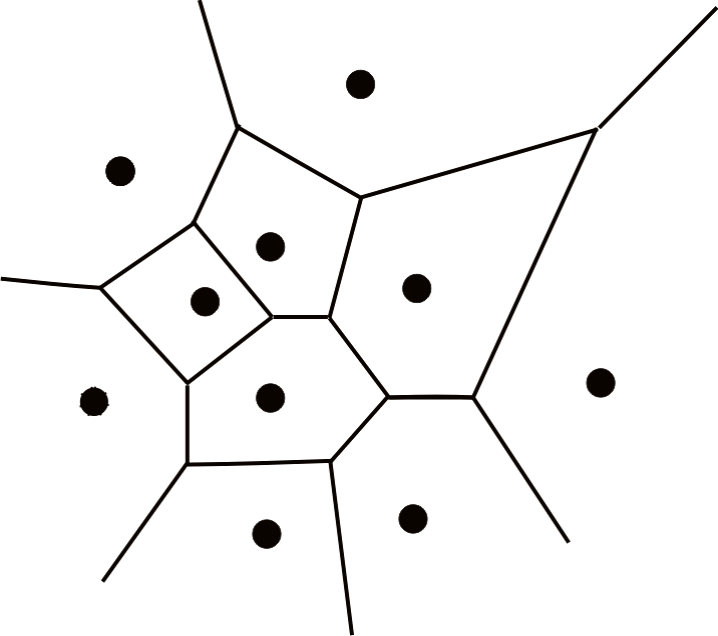
\includegraphics[scale=0.15]{voronoi}
    \caption{Example of a Voronoi diagram using euclidean distance\cite{voronoi}}
    \label{fig:voronoi}
\end{figure}


Finding the optimal solution to the k-means clustering problem in general Euclidean space is NP-hard\cite{Aloise2009}, and also NP-hard for a general number of clusters k (even in the plane)\cite{Mahajan2009}. However, running the k-means algorithm can be relatively fast so it is not uncommon to run it multiple times with different initial number of clusters and/or cluster means. In this report we do not aim to find the optimal solution, but rather to explore how great a speedup can be achieved by making a parallel implementation of the k-means algorithm.


\section{k-means algorithm}
The serial algorithm used here is an iterative solution most often referred to as simply the \textit{k-means algorithm}, or \textit{Lloyd's algorithm}\footnote{Also known as Voronoi iteration} after Stuart Lloyd who came up with the technique in 1957\footnote{His techique was not published by Bell Labs until 1982.}\cite{Lloyd}. It starts with initialization of the $k$ cluster means, and then alternates between an assignment step and an update step.

The initialization method applied here for the $k$ cluster means is Forgy Random Partition where $k$ data points are chosen at random from the initial data set. The data points in the input files were already in random order so the top $k$ points were selected. The Forgy method tends to spread the intial means out across the input space.\cite{hamerly2002alternatives}

The first of the alternating steps is the assignment step in which each data point is assigned to the cluster mean with the smallest Euclidian distance, achieving the least within-cluster sum of squares:

\begin{equation}
\begin{split}
S_i^{(t)} = \big \{& x_p : \big \| x_p - \mu^{(t)}_i \big \|^2 \le \big \| x_p - \mu^{(t)}_j \big \|^2 \ \\
& \forall j, 1 \le j \le k \big\}
\end{split}
\end{equation}

where each $x_p$ is assigned to just a single $S^t$ even though it could be assigned to more than one.

In the update step the new cluster centroids are calculated:

\begin{equation}
    \mu^{(t+1)}_i = \frac{1}{\|S^{(t)}_i\|} \sum_{x_j \in S^{(t)}_i} x_j
\end{equation}

The algorithm has converged to a \textit{local optimum} when all data points stay within their previously assigned clusters.

Each processor contains the following data structures:
\begin{itemize}
    \item an $n \times d$ array of the data points that have been assigned to that processor
    \item a $k \times d$ array of cluster means
    \item a $k \times d$ array of the total sum of $d$-dimensional vectors assigned to each of the $k$ clusters
    \item a vector of length $k$ containing the total number of points assigned to each cluster
\end{itemize}

\subsection{k-means algorithm pseudocode}

\begin{algorithm}[H]
\caption{k\_means\_clustering()}
\begin{algorithmic} 
\REQUIRE N: number of data objects
\REQUIRE K: number of clusters
\REQUIRE objects[N]: array of data objects
\REQUIRE clusters[K] array of cluster centers
\REQUIRE membership[N]: array of object memberships
\WHILE{$\delta/N > threshold$}
\STATE $\delta \leftarrow 0$
\FOR{$i \leftarrow 0 $ to $ N-1$} 
\FOR{$j \leftarrow 0$ to $K-1$} 
\STATE $distance \leftarrow  | objects[i] - clusters[i] |$
\IF{$distance < dMin$}
\STATE $dmin \leftarrow distance$
\STATE $n \leftarrow j$
\ENDIF
\ENDFOR
\IF{$memberships[i] \neq n$}
\STATE $\delta \leftarrow \delta + 1$
\STATE $membership[i] \leftarrow n$
\ENDIF
\STATE $new\_clusters[n] \leftarrow new\_clusters[n] + objects[i]$
\STATE $new\_cluster\_size[n] \leftarrow new\_cluster\_size[n] + 1$
\ENDFOR
\FOR{$j \leftarrow 0$ to $K-1$}
\STATE $clusters[j][*] \leftarrow new\_clusters[j][*] / new\_cluster\_size[j]$
\STATE $new\_clusters[j][*] \leftarrow 0$
\STATE $new\_cluster\_size[j] \leftarrow 0$
\ENDFOR
\ENDWHILE
\end{algorithmic}
\end{algorithm}


\subsection{Additions for parallelization}
In addition to the above mentioned data structures each processor in the parallel implementation contains:
\begin{itemize}
    \item a $k \times d$ array of the locally calculated total sum of vectors assigned to each cluster
    \item a vector of length $k$ containing the locally calculated total number of points assigned to each cluster
\end{itemize}

In the parallel implementation used in this report a few extra steps are required. At the start, processor 0 selects the top $k$ data points belonging to it as the initial global cluster means. Those are communicated to the other processors using \texttt{MPI\_Bcast}. 

During an iteration each processor maintains a local $k \times d$ array containing the total sum of the $d$-dimensional points assigned to each of the $k$ clusters, and a vector of length $k$ containing the total number of points assigned to each cluster. At the end of an iteration both of these arrays need to be summed across processors. This is achieved with two separate calls to \texttt{MPI\_Allreduce} using the \texttt{MPI\_SUM} functionality. Then each processor uses those to calculate the new global cluster means locally.

\section{Theoretical performance estimation}
k-means is a heuristic algorithm and there is no guarantee that it will converge to a global optimum. The results will in each case depend on the chosen $k$ and the initial cluster selection. However, the algorithm is usually very fast and analysis has shown that its smoothed running time is polynomial\cite{arthur2009k}.
The k-means (Lloyd's) algorithm spends most of its time calculating the distances between each of the data points and each of the clusters. The running time of the algorithm is $\mathcal{O}(nkdi)$, where
\begin{itemize}
    \item $n$ is the number of data points
    \item $k$ is the number of clusters
    \item $d$ is the dimensionality of each data point
    \item $i$ is the number of iterations needed until convergence
\end{itemize}
 
As such the k-means algorithm can be considered to have linear complexity. When the data does exhibit a clustering structure the algorithm can converge in relatively few iterations, quickly approximating the clusters and then achieving marginal improvements in subsequent iterations. 

The time complexity of each iteration is split into calculations and communication. 
\begin{enumerate}
    \item calculate local cluster sums: $n_{p}kd$ where $n_p$ is the number of data points belonging to processor $p$
    \item send local cluster sums: $t_{startup} + t_{data} * k * d$
    \item send local cluster counts: $t_{startup} + t_{data} * k$
    \item calculate new cluster means: $kd$ 
\end{enumerate} 

\begin{equation}
T_p = \mathcal{O}(i * (n_{p}kd + 2(t_{startup} + t_{data}k(d + 1)) + kd))
\end{equation}

\begin{equation}
T^*_s = \mathcal{O}(nkdi)
\end{equation}

The speedup can then be calculated as

\begin{equation}
\begin{split}
    S_p &= \frac{T^*_s}{T_p} \\
        &= \frac{nkdi}{i * (n_{p}kd + 2(t_{startup} + t_{data}k(d + 1)) + kd)} \\
        &= \frac{dkn}{dkn_p + 2((d+1)kt_{data} + dk + t_{startup})}
\end{split}
\end{equation}


\section{Implementation details}
The generated data sets all have 5 clusters, and in the implementation the same number of clusters are assumed. The higher the dimensionality of data becomes, the further apart the points will become. Due to this it was difficult to generate clustered data sets that would result in a similar number of iterations until convergence. This led for example to the 16-dimensional data set converging in much fewer iterations than the 8-dimensional one. For this reason the iteration count was fixed at 100 and million data points.

Due to disk space limitation in the KTH system of around 600 MB each data set was limited to 1 million data points of double-precision. 


\section{Results}
Experiments were run on Tegner on PDC. To avoid inter-node communication a maximum of 24 cores were used. Each data set had 1 million double-precision points containing 5 clusters, generated from 5 multinomial Gaussian distributions, and between 2-32 dimensions.

Table \ref{tab:wallclock} shows the wall-clock time results for different data sets and numbers of processors used. The results indicate that parallelizing k-means can be very efficient. Doubling the number of processors generally halved the run time. This is what we hoped for at the beginning of the experiment.

\begin{table}[ht]
\centering
\caption{Wall-clock time for different dimensions and number of cores}
\label{tab:wallclock}
\begin{tabular}{@{}llllll@{}}
\toprule
Cores & \multicolumn{5}{c}{Dimensions} \\ 
      \cmidrule{2-6}
                & 2   & 8   & 16   & 24   & 32   \\ \midrule
$T^*_s$ & 17.23  & 27.68   & 50.56   & 88.97    & 163.34   \\
3 & 6.06	&	9.56	&	17.63	&	35.47	&	66.84 \\
6 & 3.32	&	4.82	&	9.21	&	18.23	&	34.2 \\
12 & 1.72	&	2.58	&	5.03	&	9.5	&	17.75 \\
24 & 0.87	&	1.43	&	2.59	&	4.36	&	8.21 \\ \bottomrule
\end{tabular}
\end{table}


\begin{table}[ht]
\centering
\caption{Speedup for different dimensions and number of cores}
\label{speedup}
\begin{tabular}{@{}llllll@{}}
\toprule
Cores & \multicolumn{5}{c}{Dimensions} \\ 
      \cmidrule{2-6}
                & 2   & 8   & 16   & 24   & 32   \\ \midrule
3  & 2.44 &  2.50 &  2.86 &  2.89  &  2.84 \\
6  &  4.77 &  4.88 &  5.49 &  5.74 &  5.18 \\
12 &  9.20 &  9.36 & 10.05  & 10.72  & 10.01  \\
24 & 19.89  & 20.40   & 19.52  & 19.35 & 19.80  \\\bottomrule
\end{tabular}
\end{table}


\begin{figure}[h]
\centering
    \begin{subfigure}{0.5\textwidth}
    \centering
        \captionsetup{width=0.9\linewidth}
        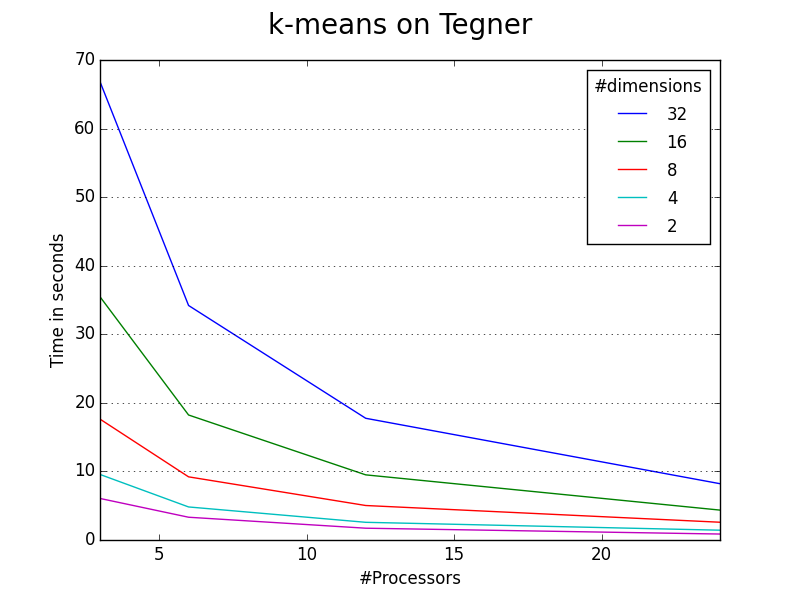
\includegraphics[width=1.1\linewidth]{img/Times}
        \caption{Wall-clock run time for different data sets and number of processors. The y-axis shows the wall clock time in seconds and the x-axis shows the number of processors for each dimension.}
        \label{fig:times}
    \end{subfigure}%
    \begin{subfigure}{0.5\textwidth}
    \centering
        \captionsetup{width=0.9\linewidth}
        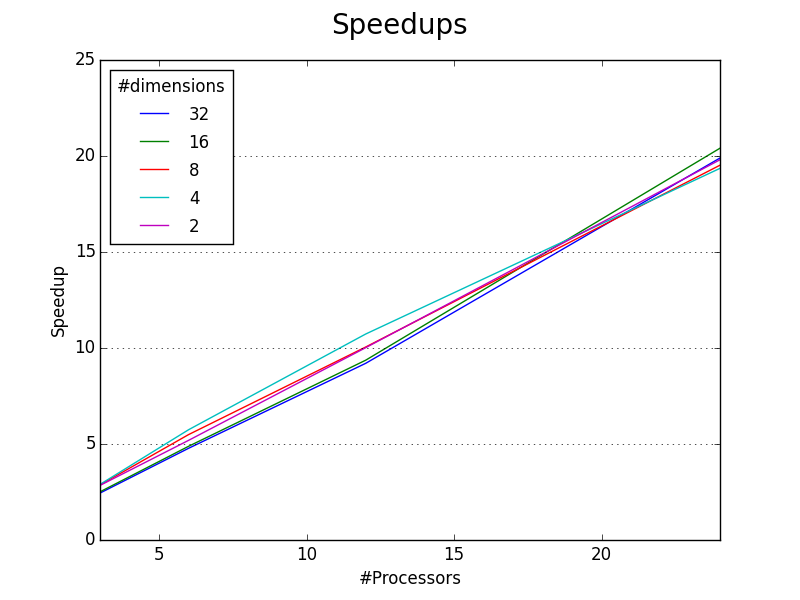
\includegraphics[width=1.1\linewidth]{img/Speedups}
        \caption{Speedup obtained using different data sets and number of processors. The y-axis is the calculated speedup using equation \ref{eq:SpeedupFormula} and the x-axis shows the number of processors tested.}
        \label{fig:speedup}
    \end{subfigure}
\caption{Graphical results for computation time and speedup.}
\label{fig:Q112_pool}
\end{figure}

Equation \ref{eq:SpeedupFormula} was used to calculate speedup. $T^*_s$ was obtained by running a sequential version of the algorithm on Tegner.
\begin{equation} 
\label{eq:SpeedupFormula}
S_P = \frac{T^*_s}{T_P}
\end{equation}

The speedup results as shown in table \ref{speedup} and figure \ref{fig:speedup} indicate that our implementation of parallel k-means has linear speedup with the number of processes. 

\section{Conclusion}
In this report we aimed to explore what level of speedup could be achieved by utilizing a parallel implementation of the k-means algorithm. Finding the optimal solution to the k-means clustering problem is NP-hard, but running the k-means algorithm can be relatively fast. It is therefore feasible to run it multiple times with different initial configurations.

We proposed a fast parallel k-means clustering algorithm and tested it on a data set of 1 million points with between 2-32 dimensions. The results show that the proposed algorithms has linear speedup the number of processors making it very feasible to run it multiple times with different initial configurations compared to a serial implementation.


\vfill
\bibliographystyle{ieeetr}%Used BibTeX style is unsrt
\bibliography{bibliography}


%% In case we get asked, here is an explanation for smoothed running time.

\begin{comment}
https://en.wikipedia.org/wiki/Smoothed_analysis

Smoothed analysis is a way of measuring the complexity of an algorithm. It gives a more realistic analysis of the practical performance of the algorithm, such as its running time, than using worst-case or average-case scenarios.

For instance the simplex algorithm runs in exponential-time in the worst-case and yet in practice it is a very efficient algorithm. This was one of the main motivations for developing smoothed analysis.

Smoothed analysis is a hybrid of worst-case and average-case analyses that inherits advantages of both, by measuring the expected performance of algorithms under slight random perturbations of worst-case inputs. If the smoothed complexity of an algorithm is low, then it is unlikely that the algorithm will take long time to solve practical instances whose data are subject to slight noises and imprecisions.
\end{comment}


\end{document}


